
The remote sensing of any atmospheric component is based on its interaction with
electromagnetic radiation. By inverting this interaction, the measured radiation
can be used to infer certain properties of this component. This chapter presents
the physical processes underlying these interactions as well as relevant
practical aspects of observing the atmosphere from space.

The first part of this chapter provides a brief introduction to radiative
transfer (RT) theory, which can be used to describe the interaction of radiation
with the atmosphere. Based on this, the principal characteristics of
observations across the electromagnetic spectrum and their sensitivity to
hydrometeors%
%
\footnote{ Hydrometeor is the collective term for the liquid and frozen particles that make
up clouds and precipitation.}%
%
are discussed. The focus is put on observations that measure radiation emitted
from the sun or the Earth and its atmosphere, so called
\textit{passive observations}.
The remaining part of this chapter then provides an overview of the types of
different satellite observations that were used in the retrieval applications
developed in this thesis.


%Doing so, requires a quantitative model of the propagation of radiation through
%the atmosphere. Such a model is provided by the physical theory of 
%Since radiative transfer theory is fundamental to atmospheric remote sensing ,
%this section provides an introduction to radiative transfer in the atmosphere.
%The focus is put on the interaction of radiation with hydrometeors. This
%presentation is mostly based on the more comprehensive texts by Mishchenko et
%al. (2002), Thomas and Stamnes (2002), and Wallace and Hobbs (2006).


\section{Radiative transfer theory}

Radiative transfer theory describes the propagation of a perfectly monochromatic
beam of light through a medium. As the beam propagates it interacts with the
medium through electromagnetic and quantum mechanical processes. Radiative
transfer theory provides a simplified model of these interactions, which is well
suited for the conditions of passive remote sensing of the atmosphere. The
following presentation is based on the more comprehensive texts
by \citet{mischenko02}, \citet{thomas02} and \citet{wallace06}.
%al. (2002), Thomas and Stamnes (2002), and Wallace and Hobbs (2006).

Electromagnetic sensors measure the mean total energy that is transferred by
electromagnetic radiation over a finite time interval. The way in which this
energy is distributed across the components of the electric field is defined as
its \textit{polarization state}. Mathematically, the polarization state of the
beam can be described using the four dimensional Stokes vector
\begin{align}
  \bm{I} &= \left [ \begin{array}{c}
    I \\
    Q \\
    U \\
    V \\
    \end{array} \right ]
\end{align}
The components $I$, $Q$, $U$ and $V$ are called the Stokes parameters and have the
unit of monochromatic energy flux per solid angle. The Stokes vector fully
describes the state of a monochromatic beam of radiation to the extent that it
can be measured by an electromagnetic sensor. Any electromagnetic
measurement can thus be derived from knowledge of the Stokes vector at the position
and orientation of the sensor. Radiative transfer theory describes how the
Stokes vector changes as it propagates through a medium and thus allows
the modeling of satellite observations of the atmosphere.

\subsection{Interactions with matter}

Radiative transfer theory distinguishes three fundamental processes through
which matter interacts with radiation. These are the emission of
electromagnetic radiation, its absorption and scattering.

\subsubsection{Emission}

At temperatures above absolute zero, all matter emits thermal radiation. Thermal
radiation is produced when molecules transition from a quantum mechanical state
of higher energy to one of lower energy causing the excess energy to be emitted
in the form of radiation. The amount of radiation that a body emits varies with
its material properties and temperature as well as the wavelength $\lambda$ of
the radiation.

In radiative transfer theory, emission from arbitrary matter is modeled using a
material-dependent emissivity vector $\vec{e}$, which relates the emission of
the material to that of a black body. A black body is an idealized body that
absorbs all incoming radiation. The intensity of the radiation emitted by a
black body at temperature $T$ and wavelength $\lambda$ is given by Planck's law
\begin{align}
B(T, \lambda) &= \frac{2 h c^2}{\lambda ^ 5}\frac{1}{e^{\frac{hc}{\lambda k_B T}} - 1},
\end{align} with $c$ is the speed of light in vacuum, $h$ the Planck
constant and $k$ the Boltzmann constant.

The emissivity vector $\vec{e}$ describes the amount of radiation that is
emitted along an infinitesimal step $ds$ along the propagation path of a beam: 
 \begin{align}
   \label{eq:emissivity}
   \vec{I}_\text{emitted} &= \vec{e} \cdot B(T, \nu)\ ds.
 \end{align}
 Eq.~\ref{eq:emissivity} provides a deceptively simple way to calculate the
 radiation emitted by arbitrary materials. It is clear that this formulation
 delegates much of the complexity of calculating the radiation emitted from a
 material to the calculation of the emissivity vector $\vec{e}$. In the
 atmosphere, $\vec{e}$ depends on the concentrations of gases, aerosols and
 hydrometeors as well as the local temperature and pressure. A significant part
 of the difficulty of calculating thermal emission from the atmosphere arises
 from determining its emissivity.



%For a material that is opaque, there is no need to integrate over the full
%volume, since only its surface will contribute to the observed emission.
%The emissivity of a surface can be described using an emissivity vector
%$\vec{e}$ in the same way as for emission from a volume, with the difference
%that its components are unitless and integration over the propagation path is
%not required.

\subsubsection{Absorption}

Absorption refers to the process of radiation being converted into internal
energy of the matter it interacts with. Mathematically, this process is
described by the absorption vector $\vec{\alpha}$, defined as the fraction of
the beam's radiation that is absorbed along an infinitesimal step of length $ds$
along its propagation path:
\begin{align}
\vec{I}_\text{absorbed} &= \vec{\alpha} \odot \vec{I} \ ds
\end{align}
Here $\odot$ denotes the element-wise product of the absorption vector and
the Stokes vector $\vec{I}$ of the incoming radiation. Absorption may be
understood as the inverse process of thermal emission. Formally, this is
expressed by Kirchoff's  law of radiation
\begin{align}
  \vec{\alpha} &= \vec{\epsilon},
\end{align}
which states that the absorption vector is identical to the emissivity vector
defined in Eq.~\ref{eq:emissivity}. This law is applicable to all matter in the
atmosphere given that it is in a state of local thermal equilibrium (LTE). LTE
occurs when the density of matter is sufficiently high so that the population
rates of energy states above the ground state are determined by thermal
collisions rather than the absorption of radiation. This decouples the emission
of radiation from the radiation field itself, allowing the simplified treatment
of matter as thermal emitters with the emission rates independent of the
radiation field. LTE is a valid assumption for radiative transfer in the
troposphere.

\subsubsection{Scattering}

Scattering describes the effect of inhomogeneities in the medium on the
propagation of the beam. When a plane-parallel electromagnetic wave encounters
such inhomogeneities, it is scattered in all directions. Mathematically, the
scattering of a beam of light propagating in direction $\vec{n}$ into the
direction $\vec{\hat{n}}$ is described by the phase matrix
$\mat{Z}(\vec{\hat{n}}, \vec{n})$:
\begin{align}
  \vec{I}_\text{scattered}(\vec{\hat{n}}) &= \mat{Z}(\vec{\hat{n}}, \vec{n}) \vec{I}(\vec{n})
\end{align}
Since parts of the energy transported by the beam are deviated from its
propagation path, its intensity is decreased. As it propagates through the
medium, the intensity of a beam is thus decreased by the effects of absorption
and scattering. The combination of these two processes is referred to
as \textit{attenuation} or \textit{extinction} and is described by the
attenuation matrix $\mat{K}$, which is the sum of the absorption vector
$\vec{\alpha}$ and the fraction of radiation scattered away from the propagation
path:
\newcommand*{\vertbar}{\rule[-1ex]{0.5pt}{2.5ex}}
\newcommand*{\horzbar}{\rule[.5ex]{2.5ex}{0.5pt}}
\begin{align}
  \vec{K} &=
  \left [ \begin{array}{cccc}
      \vertbar & \vertbar & \vertbar & \vertbar \\
      \vec{\alpha} & \vec{0} & \vec{0} & \vec{0} \\
      \vertbar & \vertbar & \vertbar & \vertbar
    \end{array} \right ]
       + \int_{\vec{\hat{n}}} d\vec{\hat{n}}\ \mat{Z}(\vec{\hat{n}}, \vec{n})
\end{align}

The strength of the scattering interaction depends on the relation of the size
of the inhomogeneities to the wavelength of the radiation. When the scale of the
inhomogeneities is much smaller than the wavelength, the effects of scattering
can often be neglected. As the relative size of the inhomogeneities increases,
the strength of the scattering increases and its effects must be taken into
account. The scattering interaction drastically complicates the modeling of the
radiative transfer because it requires taking into account the radiation that is
scattered into the line of sight from all directions. Further difficulty arises
from the dependency of the scattering properties on the shape of the
inhomogeneities, which makes it difficult to calculate the scattering
and absorption properties of scattering materials with irregular shapes.

Because of their relatively large size, scattering effects from hydrometeors
need to be taken into account across most of the electromagnetic spectrum.
Frozen hydrometeors also exhibit highly variable shapes, which makes the
calculation of their scattering properties uncertain and highly complex. These
factors make the modeling satellite observations of hydrometeors a scientific
and computational challenge.


\subsection{The radiative transfer equation}

The previous section introduced the fundamental interactions of radiation
with matter and how they are described mathematically by radiative transfer
theory. Combining the three processes of emission, absorption and scattering,
the change that a beam undergoes as it travels a distance $ds$ along its
propagation path through the atmosphere is described by the vector radiative
transfer equation (VRTE):
\begin{align}\label{eq:vrte}
  \frac{d\vec{I}(\vec{n})}{ds} &=
  -\mat{K}\vec{I}(\vec{n}) + \vec{\alpha} \cdot B_\nu(T) + \int_{\hat{\vec{n}}} d\hat{\vec{n}} \ \mathbf{Z}(\vec{n}, \vec{\hat{n}}) \vec{I}(\vec{\hat{n}}).
  \end{align}

The first term on the right hand side is the extinction term, which represents
the combined effects of absorption and scattering of radiation out of the
propagation direction, which act to decrease the intensity of the radiation
along the line of sight. The second term represents emission along the line of
propagation, with the emissivity vector $\bm{\epsilon}$ replaced by the
absorption vector $\bm{a}$ according to Kirchoff's law of thermal radiation.
The third term represents the radiation that is scattered into the line of
sight. Both of these terms act to increase the intensity of the radiation
in the beam. 

\section{Observations of hydrometeors}
%
\begin{figure}[!tbh]
  \centering
  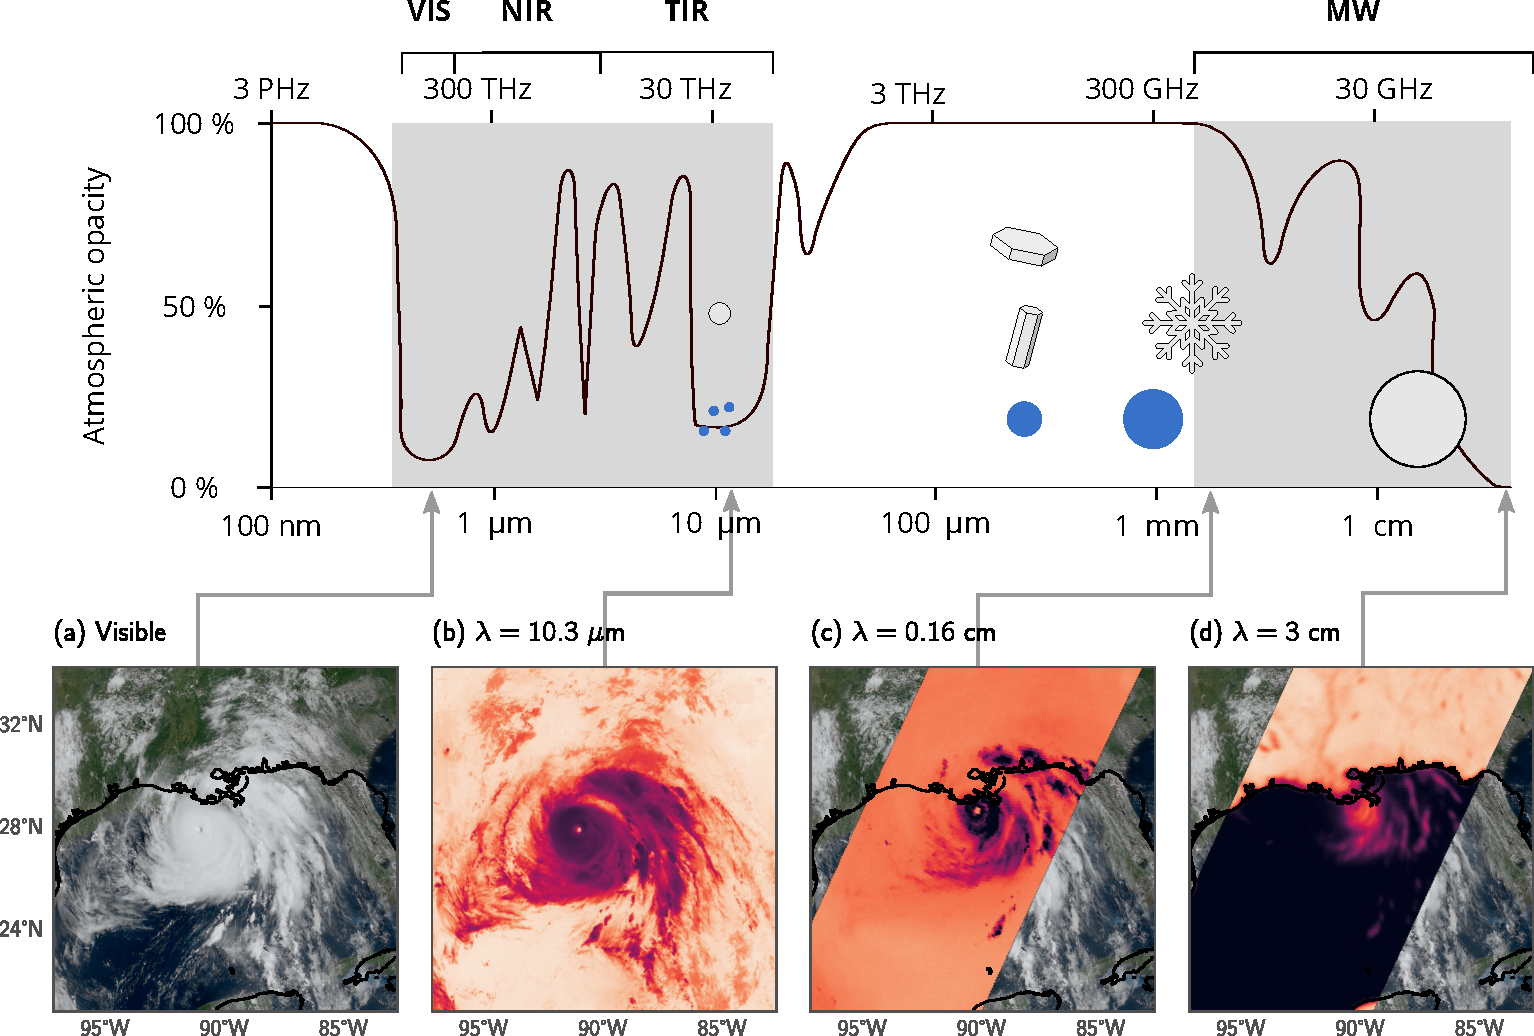
\includegraphics[width=1.0\textwidth]{spectrum_complete_no_cb}
  \caption{Overview of the electromagnetic spectrum used for hydrometeor
    retrievals. The black curve in the top panel shows the variation of the
    atmospheric opacity across the spectrum. Principal classes of hydrometeors
    are drawn at the wavelength corresponding to their representative size.
    Liquid hydrometeors are drawn in blue, while frozen hydrometeors in gray.
    The four lower panels show example observations of hurricane Ida from at
    different wavelengths.}
  \label{fig:radiative_transfer:spectrum}
\end{figure}

Radiative transfer theory describes the propagation of radiation through the
atmosphere in terms of its radiative properties, which are represented by the
absorption vector $\vec{\alpha}$, the extinction matrix $\vec{K}$ and the phase
matrix $\vec{Z}$. In order to apply radiative transfer theory to gain an
understanding of remote sensing observations of the atmosphere, its composition
must be related to its radiative properties.

The radiative properties of the atmosphere are strongly dependent on the
wavelength $\lambda$ at which it is observed. The applications presented
in this thesis make use of observations from the visible to the microwave
region of the electromagnetic spectrum. To gain an understanding of the principal
properties of these observations, it is practical distinguish the following
four different wavelength domains:
\begin{description}[midpenalty=100000]
\item[Visible (VIS):] $\SI{350}{\nano \meter} \leq \lambda < \SI{720}{\nano \meter}$
\item[Near infrared (NIR):] $\SI{720}{\nano \meter} \leq \lambda < \SI{2.5}{\micro \meter}$
\item[Thermal infrared (TIR):] $\SI{2.5}{\nano \meter} \leq \lambda < \SI{20.0}{\micro \meter}$
\item[Microwave (MW):] $\SI{1}{\milli \meter} \leq \lambda < \SI{1}{ \meter}$
\end{description}
An overview of these regions within the spectrum of electromagnetic radiation is
provided in Fig.~\ref{fig:radiative_transfer:spectrum}. The top panel shows a
simplified graph of the variation of opacity of a cloud-free atmosphere, which
is defined as the fraction by which the intensity of a beam is reduced as it
propagates from the bottom to the top of the atmosphere. When viewed from a
satellite, the atmospheric opacity gives an indication of how far down into the
atmosphere a sensor can `see'. Generally, the satellite can see down to the
surface where the opacity is low, while it is sensitive only to the upper parts
of the atmosphere where it is high. Fig.~\ref{fig:radiative_transfer:spectrum}
also contains four examples observations of hurricane Ida from across the
electromagnetic spectrum, which will be used in the following to illustrate
the principal characteristics of the corresponding observations.

Observations of the atmosphere are the results of the combined effects of gases,
aerosols and hydrometeors. To gain an understanding of the information that
certain observations provide on hydrometeors, it is helpful to decompose the
contributions into a clear-sky component, which takes into account only the
effects of molecules and aerosols, and a cloudy-sky component, which takes into
account the effects of hydrometeors. As a first approximation, the clear-sky
component maybe viewed as the background upon which the hydrometeors are
observed.

\subsection{The atmospheric background}

Observations at short wavelengths differ from those at long wavelengths with
respect to the origin of the observed radiation. In the VIS and NIR regions, the
largest part of the observed radiation stems from the sun. This is because, at
these short wavelengths, black body radiation at typical atmospheric
temperatures is small compared to reflection of solar radiation. As the
wavelength increases, the intensity of solar radiation decreases while that of a
black body at atmospheric temperatures increases. At wavelengths exceeding
approximately $\SI{2.5}{\micro \meter}$, emission from atmospheric constituents
dominates the intensity of reflected solar radiation. This threshold separates
the thermal from the near infrared. At these wavelengths solar emission can
generally be neglected and all observed radiation originates from the atmosphere
itself or the Earth's surface.

The atmospheric opacity displayed in the top panel of
Fig.~\ref{fig:radiative_transfer:spectrum} corresponds to the combined effects
of absorption and extinction by gases in the atmosphere. Gases affect radiation
mostly through absorption and emission, while scattering plays a role only in
the visible range. The reason for this is the small size of the molecules
compared to the wavelengths of the radiation.

There is little absorption and molecular scattering in the visible range, which
makes the atmosphere transparent to the human eye. Satellite observations
therefore see down to the surface of the Earth where it isn't covered by clouds
(see panel (a) of Fig.~\ref{fig:radiative_transfer:spectrum}). In the near and
thermal infrared, absorption increases but is concentrated in discrete
absorption bands, which makes the opacity of atmosphere highly variable across
wavelengths. The principal gaseous absorbers in the infrared region are water
vapor, carbon dioxide and ozone. The banded structure of the atmospheric opacity
gives rise to so-called \textit{window channels}, which are channels in which
the atmospheric opacity is low. An example of such a window channel is given in
panel (b) of Fig.~\ref{fig:radiative_transfer:spectrum}. Because of the low
opacity in this channel, the radiation observed in the cloud-free regions of the
image corresponds to thermal radiation from the Earth's surface, which is
intense because of the relatively high temperatures and the high emissivity of
the land and ocean surfaces.

Molecular absorption also plays an important role in the microwave region
\footnote{For microwave applications it is common
practice to refer to wavelengths in frequency units. We will follow this
convention here but give the corresponding wavelength in parentheses.}
with significant contributions from water vapor, oxygen, nitrogen and ozone. At
the short-wavelength end of the region, the atmosphere is relatively opaque
because of absorption from water vapor. The observations show in panel (c) of
Fig.~\ref{fig:radiative_transfer:spectrum} are located close to a strong water
vapor absorption line at $\SI{183}{\giga \hertz}$
($\lambda \approx \SI{1.6}{\milli \meter}$). Because the atomsphere is fully
opaque at this wavelength, the observed thermal radiation from water vapor stems from
higher up in the atmosphere than at channels with lower opacity. This causes the
lower intensities observed in the cloud-free regions of the observations. At the
long-wavelength end of the microwave region, the opacity of the atmosphere is
low and the observations are again sensitive to the surface. As can be seen in panel
(d) of Fig.~\ref{fig:radiative_transfer:spectrum}, there is very strong contrast
between land and ocean surfaces. This is because of the different radiative
properties of land and water surfaces at these wavelengths and the angle
at which the observations are performed.

\subsection{Physical and radiative properties of hydrometeors}

The radiative properties of hydrometeors depend on their size and whether they
are in the liquid or frozen phase. Because the dielectric properties of ice and
water differ significantly across the electromagnetic spectrum, hydrometeors of
similar sizes may have drastically different radiative properties at certain
wavelength. To provide an overview of the sizes of the principal classes of
hydrometeors with respect to the observation wavelength, they are displayed in
Fig.~\ref{fig:radiative_transfer:spectrum} at the wavelengths corresponding to
their approximate sizes. Liquid hydrometeors are identified using blue coloring,
while white corresponds to frozen hydrometeors.

Among the smallest hydrometeors are liquid cloud droplets with typical sizes
around $\SI{5}{\micro \meter}$. At sizes of around $\SI{25}{\micro \meter}$,
water drops become large enough to fall out of the clouds. Small, precipitating
liquid droplets that range in size from $25$ to $\SI{250}{\micro \meter}$ are
referred to as drizzle. Larger drops are classified as rain, whose typical
size is around $\SI{1}{\milli \meter}$ but can become as large as
$\SI{5}{\milli \meter}$.

At temperatures below $\SI{0}{\celsius}$ ice crystals can form in the
atmosphere. Their sizes range from $\SI{1}{\micro \meter}$ to
$\SI{1.5}{\milli \meter}$ with typical sizes around $\SI{100}{\micro \meter}$.
Snow flakes are aggregates, which form through the collision of ice crystals.
These range in size from hundreds of micrometers to several centimeters. When
snowflakes collide with liquid drops at temperatures below $\SI{0}{\celsius}$,
the liquid drop freezes upon the snowflake causing it to grow. This process is
called riming. Heavily rimed snowflakes are referred to as graupel and have
typical sizes of around $\SI{1}{\centi \meter}$. Finally, the largest
hydrometeors are hailstones, which form only in strong thunderstorms and but can
reach sizes of up to $\SI{10}{\centi \meter}$$.


%Most observations of clouds are affected not only by the clouds themselves but
%also by other constituents of the atmosphere. In the following, we will
%therefore first discuss observations without clouds, so called \textit{clear
%  sky} observations, as these form the background for the observations of
%hydrometeors. This is followed by a discussion of the observable effects of
%hydrometeors on the observations, which gives rise to the signal in the
%\textit{all-sky observations} that can be used to infer the physical properties
%of hydrometeors.

%\subsection{The Earth's surface}
%
%The characteristics of the Earth's surface vary considerably across the
%electromagnetic spectrum. In the visible range, the surface absorbs large parts
%of the radation. The darkest surfaces are the ocean which absorbs around
%$\SI{95}{\percent}$ of the incoming radiation. Bare land surface and forests are
%considerable brighter but still absorb most ($\approx \SI{75}{\percent}$) of the
%incoming radiation. In contrast to that, snow and ice covered surface reflect
%nearly all of the incoming radiation and thus appear very bright.
%
%In the infrared region of the electromagnetic spectrum the emissivity of the Earth surface
%increases significantly. For wavelengths between $3$ and $\SI{20}{\micro \meter}$ the emissivity
%of most surface types is larger than $0.9$. At these wavelengths the surface is very effective at
%emitting and absorbing radiation and there is little contrast between different surface types.
%
%In the microwave region surface emissivity patterns are more complex. Emissivity
%from land is relatively high, while emissivity from water surfaces is low. The
%contrast between land and surface increases with the wavelength. Emissivities
%from snow and ice are lower than that of most bare land surface but higher than
%that of water. The emissivity furthermore depends on the viewing angle and the
%polarization of the radiation.
%
%While these general tendencies are helpful for a qualitative analysis of
%satellite imagery, it should be noted that they only provide a rough
%characterization of the behavior of the Earth's surface across the
%electromagnetic spectrum. Accurate, quantitative modeling of surface
%emissivities is still an unsolved problem and thus remains an area of
%active research.

\subsection{Cloudy sky}

Due to their comparably large sizes, the scattering effects of hydrometeors need
to be taken into account across most wavelengths from the VIS to the MW regions.
In the VIS and NIR there is little absorption from either water or ice.
Hydrometeors thus mostly deviate radiation from its propagation path without
significantly decreasing its intensity. Clouds observed at these wavelengths
typically appear bright because the solar radiation  scattered back towards
the sensor is much more intense than reflection from the surface.

In the FIR region, both water and ice are strongly absorbing. Because the
ambient temperature decreases with altitude in the troposphere, the intensity of
the radiation that is emitted by a cloud is related to its altitude. The effect
of this is clearly visible in panel (b) of
Fig.~\ref{fig:radiative_transfer:spectrum}. The clouds which appear uniformly
white in the natural color composite exhibit  more structure in the
observations at $\lambda=\SI{10.3}{\micro \meter}$. The lowest intensities are
observed close to the center of the hurricane where the clouds extend highest
into the atmosphere.

In the microwave region, absorption from ice is generally much weaker than that
from liquid water. Frozen hydrometeors therefore interact with radiation
primarily through scattering. However, due to the relatively large wavelengths
of microwave observations, significant scattering effects are limited to snow,
hail and graupel and frequencies above $\SI{50}{\giga \hertz}$
($\lambda \approx \SI{6}{\milli \meter}$) . Because they are only sensitive to
large hydrometeors, only clouds that produce snow are visible in the
observations at $\SI{183}{\giga \hertz}$
($\lambda \approx \SI{1.6}{\milli \meter}$).

For passive observations the scattering from hydrometeors at frequencies below
$\SI{50}{\giga \hertz}$ can be neglected. The principal interaction with
hydrometeors is therefore thermal emission and absorption from liquid cloud
droplets and precipitation. Since water surfaces have low emissivities at these
wavelengths, emission from liquid hydrometeors causes a distinct signal in the
observations. Over ocean, the thermal emission from the rain in the hurricane is
clearly visible in the observations at $\SI{10}{\giga \hertz}$  shown in
panel (d) of Fig.~\ref{fig:radiative_transfer:spectrum}.

\section{Satellite observations}

As the discussion in the previous section showed, observations at different
wavelengths contain different information on hydrometeors. In addition to that,
the potential of satellite observations to characterize hydrometeors from space
depends the type of sensor as well as its temporal and spatial resolution. Due
to the technical complexity of operating specialized sensors in space, the
availability of observations and their characteristics are ultimately determined
by a trade-off between technical and financial constraints on one side and
scientific value on the other. The following section briefly reviews the
principal sensors types and satellite platforms that are commonly used for the
remote sensing of hydrometeors as well as the principal characteristics of
the observations that they provide.

\subsection{Sensor types}

The above discussion of radiative transfer in the atmosphere focused on
observations of radiation that originates either from the sun or the Earth and
its atmosphere. Sensors that measure these types of radiation are called passive
sensors because they do not emit any radiation themselves. \textit{Active
sensors}, on the other hand, emit radiation and measure how much of that
radiation is scattered back to the sensor. The active sensors that are used for
the remote sensing of hydrometeors are mainly radars and lidars. These sensors
measure the time of travel between of the radiation, which can be used to
infer the distance from the detector in addition to the intensity of the
reflected radiation. This allows them to profile the atmosphere along the line
of sight, leading to much higher vertical resolution than what can be achieved
with passive sensors.

From an observational perspective, the principal difference between radars and
lidars are the wavelengths at which they operate. Lidars make use of radiation with
relatively short wavelengths, which makes them sensitive scattering from
molecules, aerosol and hydrometeors. In contrast to that, radars operate at MW
wavelengths, which makes them sensitive to scattering only from hydrometeors.
Because they emit a powerful beam of radiation, active sensors are much more
sensitive to the scattering from small particles than their passive
counterparts because.

An example of radar observations from the Cloud Profiling Radar
(CPR, \citeauthor{tanelli08}, \citeyear{tanelli08}) on the CloudSat satellite is
shown in Fig.~\ref{fig:radiative_transfer:cloud_sat}. Because it was designed to
study clouds, the CPR operates at a relatively high frequency of
$\SI{94}{\giga \hertz}$. This makes it sensitive not only to precipitation but
also clouds. For these specific observations, the satellite passed directly over
the eye of the hurricane, which is clearly visible in the vertically resolved
observations.

\begin{figure}
\centering
\includegraphics[width=\textwidth]{hurricane_nicole_cloudsat}
\caption{
Radar observations of hurricane Nicole from 2016-10-12 at
17:55 UTC recorded by the CPR on the CloudSat satellite.
}
\label{fig:radiative_transfer:cloud_sat}
\end{figure}

The disadvantage of active sensors is that the horizontal extent of their
observations in the across the direction of movement, i.e. the width of
their \textit{swath}, is typically very low. This severely reduces the spatial
coverage of the observations and leads to very long times between consecutive
overpasses for a fixed position on Earth.

\subsection{Resolution and coverage}

In addition to the information content that observations can provide on
hydrometeors, their ability to resolve spatial and temporal variability as well
as how much of the globe they cover are important characteristics, which
influence their suitability for different applications.

The orbit in which a satellite is placed plays an important role in determining
these characteristics. For earth observations, two principal classes of orbits
can be distinguished: Geostationary and low-Earth orbits. Satellites in
geostationary orbit rotate around the Earth at the same angular velocity as the
Earth rotates around its axis. This allows them to hover over the same position
on the Earth's surface. Since the field of view of the satellite is constant, it
can provide observations with high temporal resolution at all locations below
the satellite. This makes these satellite suitable for many near real-time
applications in weather forecasting.

The disadvantage of geostationary platforms is their long distance from the
Earth, which is around $\SI{36000}{\kilo \meter}$. Since the spatial resolution
of microwave sensors is limited by the long wavelengths of the radiation, they
are currently not deployed on these platforms. Geostationary satellites
therefore typically carry VIS and IR sensors, which can produce observations at
very high spatial resolutions. Besides that, their orbits restricts them to
locations of the equator. The resulting viewing geometry causes the
resolution to degrade with increasing latitudes and makes the observations
unsuitable for observations at very high latitudes.

A common type of low-Earth orbit used for Earth observing satellites are polar
orbits in which the satellite passes above or nearly above the poles. The
rotation of the Earth between consecutive orbits allows these satellites to
achieve global coverage. The low altitude of these orbits ($300
- \SI{1000}{\kilo \meter}$) makes them suitable also for microwave sensors but
decreases the spatial coverage of the sensor. The swaths of sensors in low-Earth
orbits are typically limited to a few thousand kilometers in width. Depending on
the exact size of the field of view and the location on Earth, the time between
consecutive overpasses for a fixed position can be as high as $\SI{12}{\hour}.

Fig.~\ref{fig:remote_sensing:viewing_geometries} shows the field of views of the
Advanced Baseline Imager on the Geostationary Operational Environmental
Satellite (GOES) 16 and the Global Precipitation Measurement (GPM) Microwave
Image (GMI) on the polar-orbiting GPM core observatory satellite. The
observations from both satellites are projected onto the corresponding location
on the Earth. This illustration clearly shows the differences that the satellite
orbit makes for the observations. While the geostationary satellite can
permanently observe a large part of the hemisphere below it, the polar orbiting
satellite sees only a comparably thin stripe of the globe.

\begin{figure}[!hbpt]
  \centering
  \includegraphics[width=0.8\textwidth]{viewing_geometries}
  \caption{Viewing geometries of geostationary and polar-orbiting satellites
  drawn to scale. The illustration shows geo-located satellite observations from
  the GOES 16 geostationary satellite in purple and from the polar-orbiting GPM
  core observatory in orange. The spheres mark the instantaneous satellite
  positions.}
  \label{fig:remote_sensing:viewing_geometries}
\end{figure}

\subsection{Synergies}
\label{sec:radiative_transfer:synergies}

Because of the specific strengths of different sensor types and satellite
platforms, leveraging the full potential of available satellite data often
involves exploiting synergies between different observation types. An example of
this is the Global Precipitation Measurement (GPM, \citeauthor{hou14},
\citeyear{hou14}). The aim of this joint mission lead by NASA and the Japanese Space
Agency is to provide accurate, global measurements of precipitations with a
temporal resolution a few hours. The mission comprises a dedicated precipitation
satellite, the core observatory, which carries a passive microwave sensor, the
GPM Microwave Imager (GMI) and a precipitation radar. The combination of the
observation from these two dedicated precipitation sensors are used to produce the
most accurate space-borne measurements of precipitation that are currently
available.

However, because of the narrow swath of the radar, the measurements alone are
too sparse to be useful for many applications. To overcome this, the GPM mission
makes use of an opportunistic constellation of passive microwave sensors. This
constellation consists mostly of operational meteorological sensors, whose
primary purpose is the provision of observations for weather forecasting.
However, due to their reliance on microwave observations, they are also
sensitive to precipitation. The high-accuracy retrievals from the combined
observations provided by core observatory provides a reference standard, which
is used for the development of the retrievals from the passive sensors of the
GPM constellation.

The constellation currently comprises nine sensors including GMI. A snapshot of
these sensors in orbit is shown in
Fig.~\ref{fig:radiative_transfer:gpm_consteallation}. From the satellite swaths
drawn on the surface of the Earth it becomes clear that the constellation
greatly increases the spatial coverage of the measurements. The crossing of the
swaths of the GMI on GPM and the Advanced Technology Microwave Sounder (ATMS) on
Suomi NPP also shows the complementary properties of the different sensors of
the constellation. GMI has a relatively narrow swath and high resolution. The
swath of ATMS is almost three times as wide but also has a clearly lower spatial
resolution.

The retrieval from the passive microwave sensors are finally combined with
observations from geostationary satellites and rain gauges to provide global
precipitation measurements with half-hourly resolution. The resulting Integrated
Multi-sattelite Retrievals for the Global Precipitation Measurement (GPM)
Mission (IMERG, \citeauthor{huffman20}, \citeyear{huffman20}) is widely
considered the state of the art of instantaneous, global precipitation
measurement By integrating observations retrievals from a dedicated
precipitation satellites, a constellation of passive microwave diverse sensor
characteristics as well as geostationary observations and ground measurement,
the GPM mission maximizes the potential of available precipitation data.


\begin{figure}[!hbpt]
\centering
\includegraphics[width=0.4\textwidth]{gpm_constellation}
\caption{
Currently operational passive microwave sensors of the GPM constellation in
orbit around the Earth (drawn to scale) on 2022-04-19 11:26:00 UTC. Black
spheres show the location of the satellites and their names. Orange coloring on
the Earth's surface show for each sensor the observations closest to
$\SI{89}{\giga \hertz}$. Note that only six of the currently ten operational
sensors are visible.
}
\label{fig:radiative_transfer:gpm_constallation}
\end{figure}



%\subsection{Example: Satellite observations of Hurricane Ida}

%Figure~\ref{fig:radiative_transfer:observations} illustrates the different types
%of observations used for the remote sensing of hydrometeors using observations
%of Hurricane Ida shortly before landfall on August 30, 2021. The first row of
%panels shows observations derived from the Advanced Baseline Imager on the GOES
%16 geostationary satellite. Panel (a) shows a natural color composite, which
%combines observations from 3 channels from the VIS and NIR to create an image
%emulating human color vision. Panel (b) shows observations from the NIR.
%Differences in the dielectric constant of water and ice cause ice clouds to
%absorb incoming solar radiation much more strongly than water clouds. The high
%ice clouds that cover the Hurricane therefore appear much darker than in the RGB
%image. Panel (c) shows observation from a window channel in the FIR. Since it is
%a window channel, most of the radiation observed in cloud free areas stems from
%the Earth's surface and thus appear bright. Where clouds are present the
%observed brightness temperatures are closely related to the atmospheric
%temperature at the altitude of the cloud and thus colder than the surface.
%
%Panel (c) and (d) show passive microwave observations at $\SI{18.7}{\giga
%  \hertz}$ and $\SI{166}{\giga \hertz}$. At the low microwave frequency
%only the a thermal emission from precipitation in the hurricane is visible over
%the cold ocean surface, while the clouds overland yield no signal. At the higher
%microwave frequency, the surface is not visible due to emission from water
%vapor. Scattering by snow particles causes a cold scattering signal from the
%thickest clouds around the Hurricane.
%
%Finally, panel (e) shows Ku-band radar reflectivities from the GPM
%dual-frequency precipitation radar along a vertical cross section of the
%Hurricane. The signal in the radar observations is the amount of energy that is
%reflected back to the sensor. Due to the relatively low frequency of the
%radar, it is only sensitive to large, precipitation hydrometeors.
%
%
%\begin{figure}
%  \centering
%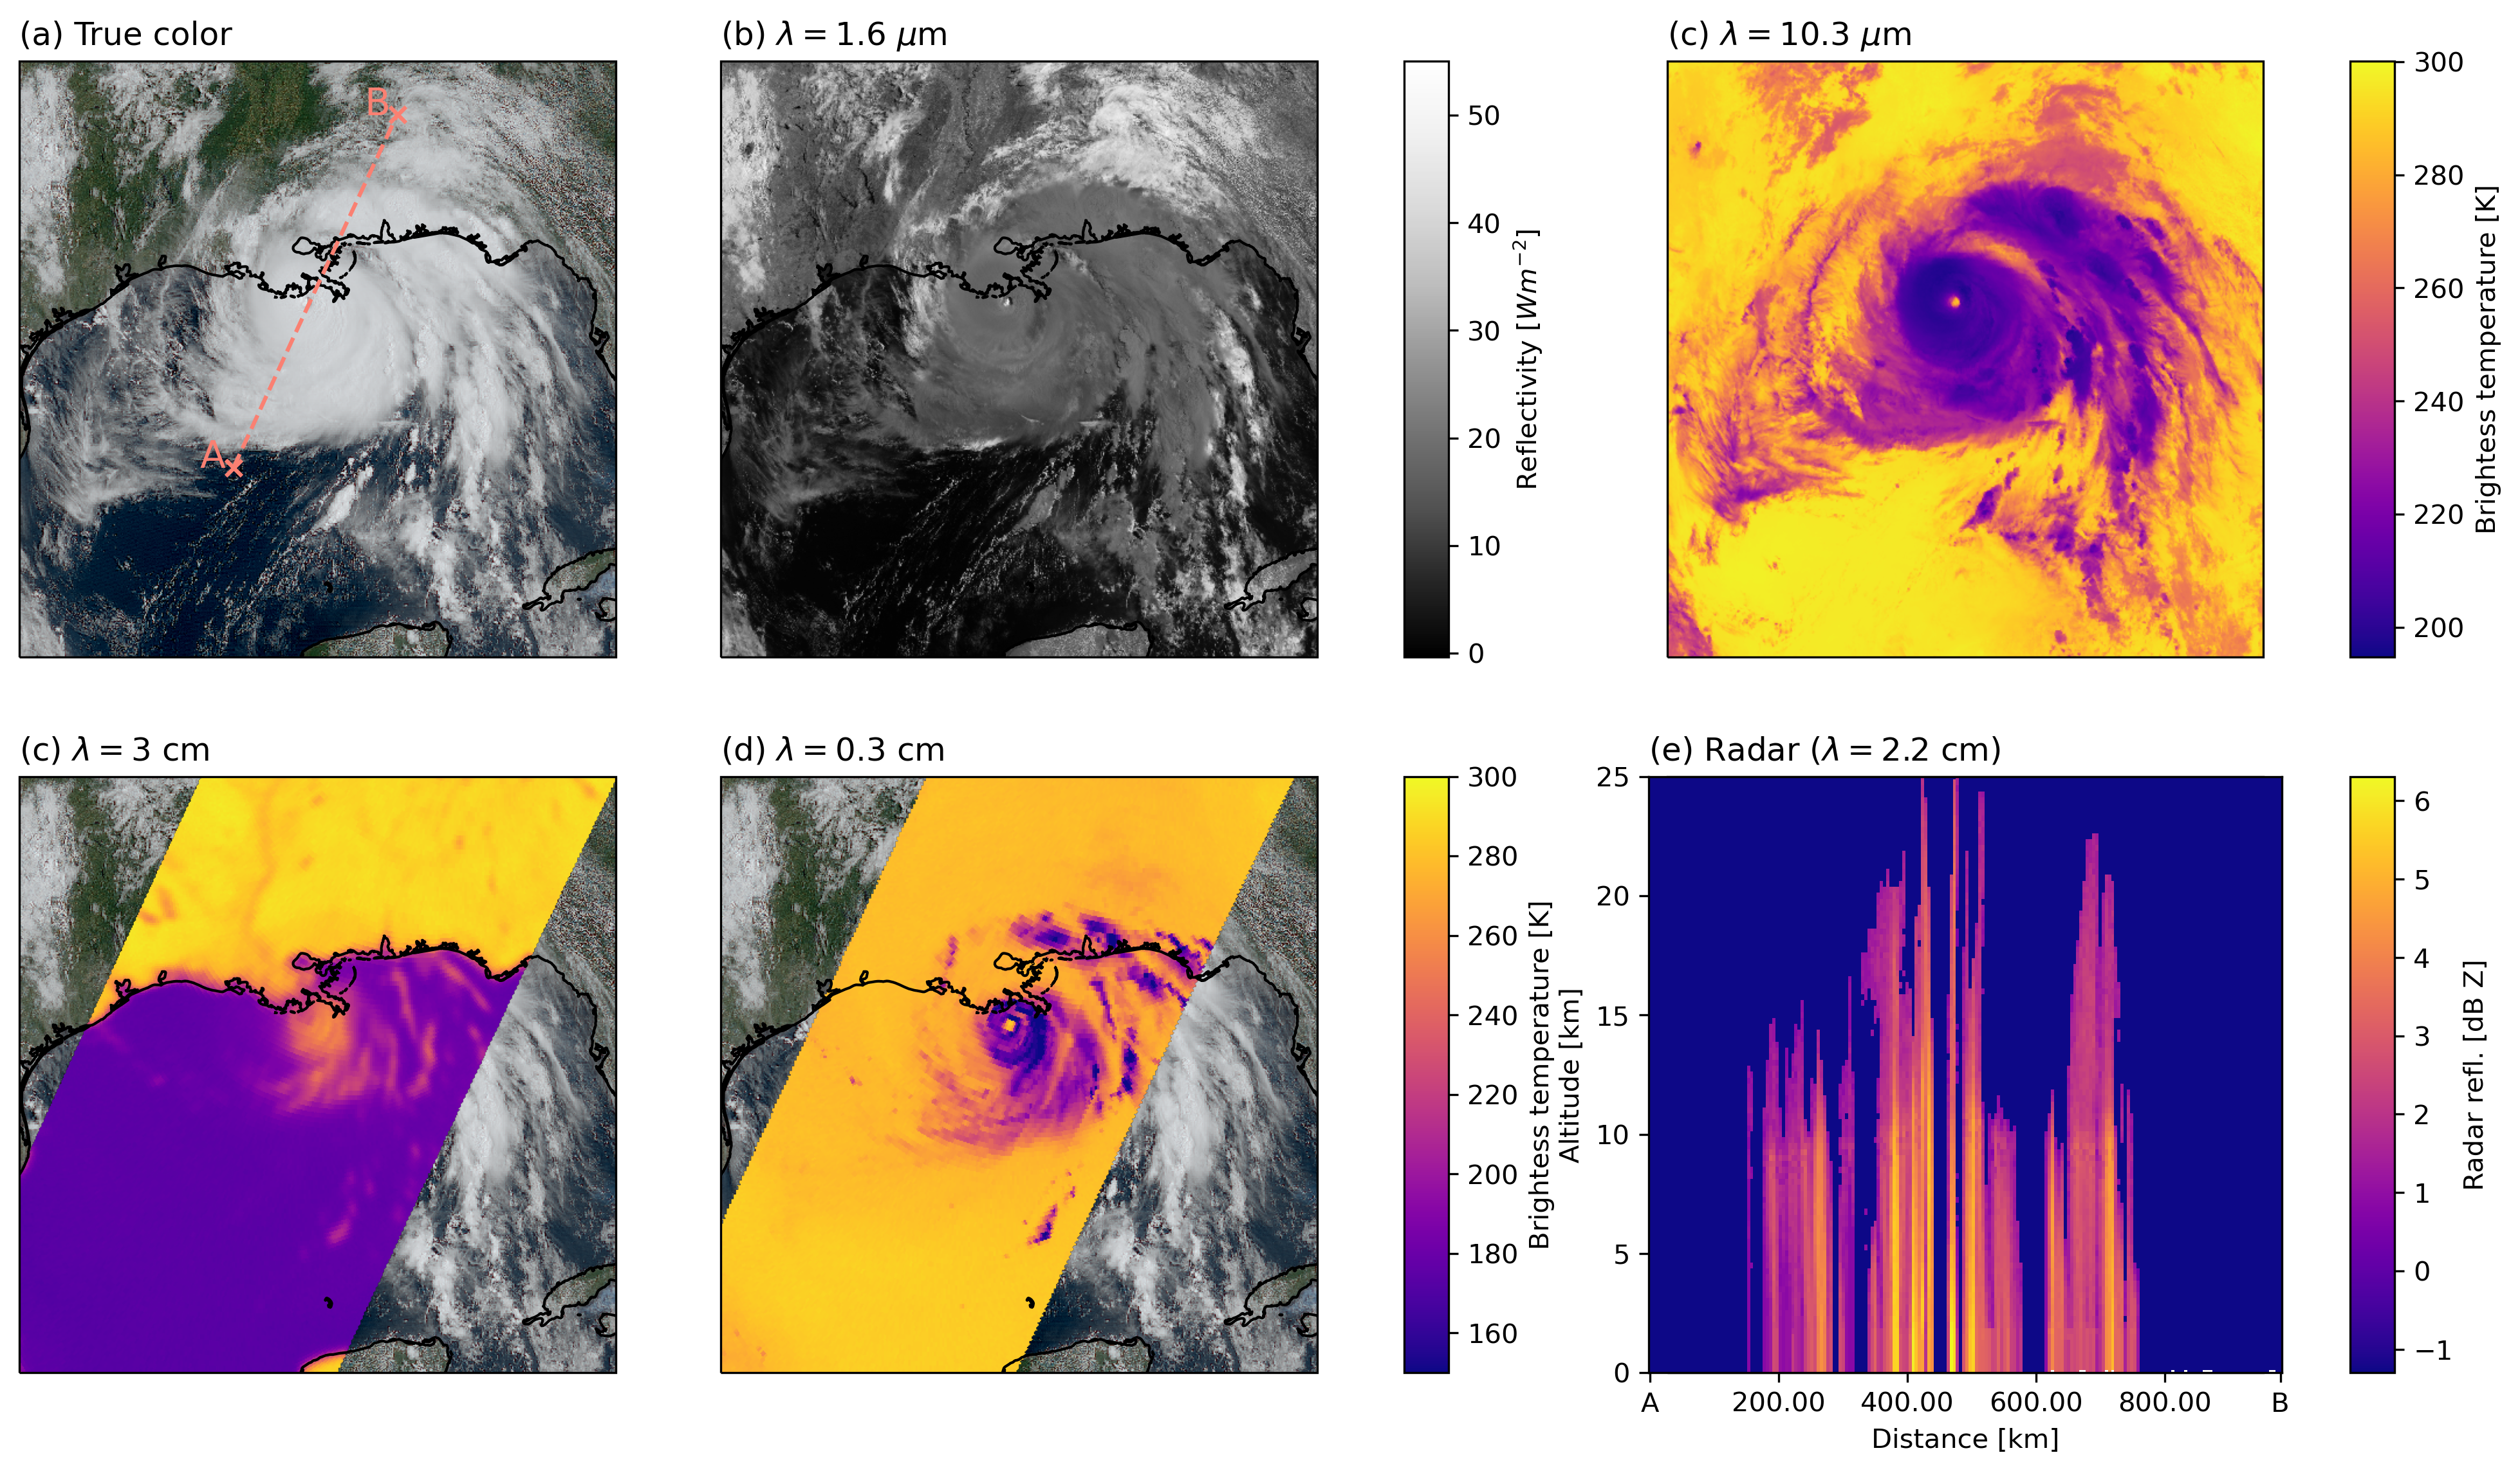
\includegraphics[width=\textwidth]{observations}
%\caption{Satellite observations of Hurricane Ida on 2021-08-29 15:09 UTC.
%  Panels (a), (b), (c) show observations from the VIS and IR regions obtained
%  by the Advanced Baseline Imager on the GOES 16 geostarionary satellite.
%  Panels (d) and (e) show passive microwave observations from the GPM microwave
%  imager. Panel (f) shows the curtain of radar reflectivity measured by the GPM dual-frequency

%  precipitation radar (DPR) along the dashed line shown in panel (a).}
%\label{fig:radiative_transfer:observations}
%\end{figure}
